
\documentclass[
12pt,
a4paper,
bibliography=totocnumbered, %Literaturverzereichnis als Eintrag ins Inhaltsverzeichnis
twoside, %Zweiseitiger Druck
BCOR=1cm, %Platz zum Lochen
%oneside, %Einseitiger Druck
]{scrartcl}

\usepackage{geometry}

\usepackage[default]{fontsetup}
%\usepackage[onehalfspacing]{setspace}

\usepackage[ngerman]{babel}
\usepackage[babel=true,german=quotes]{csquotes}

\usepackage{microtype}
\usepackage{mleftright}
%\newcommand{\Le}{\mleft}
%\newcommand{\Ri}{\mright}
\usepackage[no-script, no-scriptscript, no-inner, no-close]{innerscript}

% Mathepakete (unicode-math ersetzt amssymb, amsfonts etc.)
\usepackage{amsmath,amsthm}
\usepackage{mathtools}
\usepackage{fixdif,derivative}
\usepackage{physics2}
\usephysicsmodule{ab.legacy}

\usepackage{unicode-math}
\setmathfont{NewCMMath-Book}
\setmathfont{NewCMMath-Book}[range=cal, StylisticSet=1]
\setmathfont{NewCMMath-Book}[range=scr]

\usepackage{siunitx}
\sisetup{detect-weight=true, detect-family=true,locale=DE,range-phrase={\,bis\,},list-final-separator ={\,\linebreak[0] \text{und}\,},separate-uncertainty=true,per-mode = symbol-or-fraction}
%\SI[per-mode = fraction]{1}{\meter\per\second} erzwingt auch im Fließtext die Bruchdarstellung.
\DeclareSIUnit\curie{Ci}%Zusätzliche Einheit definieren

\usepackage{tabularx, booktabs, multirow}
\usepackage{array}
\usepackage{enumitem}
\usepackage{float}
\usepackage{graphicx}
\usepackage{xurl}

\usepackage[final]{pdfpages}
\usepackage{framed, color} %Framed: Paket, mittels dessen ein Rahmen um einen Bereich definiert werden kann. Color: Lässt Farbdarstellung in Schrift, Hintergrund etc. zu

\usepackage{scrlayer-scrpage} %Header für die KOMA-script-Klasse

%\usepackage[square,numbers]{natbib}
\usepackage{subfigure} %Mehrere Bilder in einer Figure-Umgebung

\usepackage[bookmarks,colorlinks=true]{hyperref}
\hypersetup{
	colorlinks,
	linktocpage,
	citecolor=black,
	filecolor=black,
	linkcolor=black,
	urlcolor=black,
	pdftitle=X,
	pdfauthor=JM-VS
}

\usepackage[backend=biber, style=chem-angew]{biblatex}
\addbibresource{lit.bib}

\numberwithin{equation}{section} % Die Nummerierung von Gleichungen bekommt die jeweilige Section-Nummer als Präfix

\setlength{\parindent}{0pt} %Einrücktiefe von neuen Absätzen
\setlength{\parskip}{6pt} %Abstand von Absätzen

\pagestyle{scrheadings}%Kopf und Fußzeilen
\ohead{\textbf{\GRUPPENNR\ - \VERSUCHSNR}} %Header oben links auf linker Seite (ungerade Seitenzahl) und oben rechts auf rechter Seite (gerade Seitenzahl), beinhaltet gruppennummer und Versuchskürzel. Im Fall eine einseitigen Dokuments: Header oben rechts
\ihead{\VerfasserEINS\;\&\;\VerfasserZWEI} %Header oben rechts auf linker Seite und oben links auf rechter Seite. Beinhaltet die Namen der Verfasser. Im Fall eine einseitigen Dokuments: Header oben links!
\ofoot{\thepage} %Footer unten links auf linker und unten rechts auf rechter Seite, enthält die jeweilige Seitenzahl. Im Fall eines einseitigen Elements: Footer unten rechts!
\cfoot{\empty} %Mittig unten im Footer soll nichts eingetragen werden
\ifoot{\empty} %Footer unten rechts auf linker und unten links auf rechter Seite. Hier ebenfalls leer.

\newcommand{\tz}{T_{\text{II}}}
\newcommand{\ts}{T_{\text{S}}}
\newcommand{\tgl}{T_{\text{gl}}}
\newcommand{\tgeg}{T_{\text{geg}}}
\newcommand{\omz}{\omega_{\text{II}}}
\newcommand{\omgl}{\omega_{\text{gl}}}
\newcommand{\omgeg}{\omega_{\text{geg}}}
\newcommand{\kB}{k_{\text{B}}}

% Hier können die individuellen Anpassungen vorgenommen werden, die sich auf das Titelblatt und die Kopfzeilen auswirken.

\newcommand{\VERSUCHSDATUM}{24.09.2025}
\newcommand{\PROTOKOLLDATUM}{\today}

\newcommand{\VerfasserEINS}{Julian Molt}
\newcommand{\MatNoEINS}{3803097}
\newcommand{\StudiengangEINS}{Physik}

\newcommand{\VerfasserZWEI}{Valentin Stopper}
\newcommand{\MatNoZWEI}{3774391}
\newcommand{\StudiengangZWEI}{Physik}

\newcommand{\BETREUER}{Lara Zaiser}
\newcommand{\GRUPPENNR}{A-016}

\newcommand{\VERSUCHSNR}{M23}
\newcommand{\VERSUCHSNAME}{Gekoppelte Pendel}

\newcommand{\lh}{\ell_{\mathrm{H}}}
\newcommand{\ls}{\ell_{\mathrm{S}}}


\begin{document}

\thispagestyle{empty}

\begin{titlepage}

	\begin{center}
		\Huge{\textbf{\VERSUCHSNR\ -- \VERSUCHSNAME}}\\
		\vspace{10mm}
		\Large{Protokoll zum Versuch des Physikalischen Praktikums I von \\ \textbf{\VerfasserEINS\;\& \VerfasserZWEI}}\\
		\vspace{10mm}
		\Large{Universität Stuttgart}\\
	\end{center}
	\vspace{1cm}
	\begin{center}
		\begin{tabular}{ll}
			\large{Verfasser:}		& \large{\VerfasserEINS\;(\StudiengangEINS),} \\
			& \large{\MatNoEINS} \\
			\vspace{0cm}\\
			& \large{\VerfasserZWEI\;(\StudiengangZWEI),} \\
			& \large{\MatNoZWEI} \\
			\vspace{0cm}\\
			\large{Gruppennummer:}	& \large{\GRUPPENNR} \\
			\vspace{0cm}\\
			\large{Versuchsdatum:}	& \large{\VERSUCHSDATUM} \\
			\vspace{0cm}\\
			\large{Betreuerin:}		& \large{\BETREUER}
		\end{tabular}
	\end{center}
	\vspace{15mm}

	\begin{center}
		Stuttgart, den \PROTOKOLLDATUM
	\end{center}

\end{titlepage}

\thispagestyle{empty}

\tableofcontents

\clearpage %Neue Seite, davor werden alle noch ausstehenden Grafiken/Tabellen platziert.

\renewcommand{\thepage}{\arabic{page}}
\setcounter{page}{1}


% Die erste eckige Klammer ist optional, die darin angegebene Bezeichnung steht im Inhaltsverzeichnis anstelle des hinteren (längeren) Namens.
\section[Versuchsziel]{Versuchsziel und Versuchsmethode}



\section{Grundlagen}

Eine Schwingung ist in der Physik eine Bewegung, die sich periodisch wiederholt. Sie wird wesentlich durch zwei Größen charakterisiert: Die Amplitude, welche die maximale Auslenkung aus der Ruhelage ist und die Frequenz, welche der Kehrwert der Schwingungsdauer ist. Die Schwingungsdauer ist die Zeit, die das System benötigt, um wieder in den selben Zustand zu kommen. Die harmonische Schwingung ist eine spezielle Schwingung, bei der die Rückstellkraft proportional zur Auslenkung ist, wodurch die Schwingung sinusförmig abläuft.

Ein klassisches schwingungsfähiges  System ist ein Pendel. Unterschieden wird zwischen mathematischen und physikalischen Pendeln, wobei das mathematische eine Punktmasse betrachtet, die an einer masselosen Aufhängung schwingt. Beim Physikalischen werden hingegen alle Massen und ihre räumlichen Ausdehnungen durch das Trägheitsmoment berücksichtigt.

Werden zwei Pendel gekoppelt, können diese wechselwirken und beeinflussen dann jeweils ihre Bewegungsgleichungen, die als ein paar gekoppelter Differenzialgleichungen vorliegen:
\begin{align}
	J\ddot{\psi_1} &= -Mg\ls\psi_1 - D_{\text{F}}\lh^2(\psi_1-\psi_2)\\
	J\ddot{\psi_2} &= -Mg\ls\psi_2 - D_{\text{F}}\lh^2(\psi_2-\psi_1)
\end{align}
Sie setzen sich zusammen aus den rückstellenden Drehmomenten der Gewichtskraft und der Federkraft. Die Schwerpunktmasse \(M\) ergibt sich aus der Summe über alle Teilmassen \(m, m_{\text{H}}, m_{\text{St}}\) und für ihren Abstand zur Drehachse gilt \(\ell_{\text{S}} = \frac{Lm+l_Hm_H+0,5L_{St}m_{St}}{M}\).

Mit den Kreisfrequenzen \(\omega_0^2=\frac{Mgl_s}{J}\)  und  \(\Omega^2=\frac{D_Fl_H^2}{J}\) ergibt sich:
\begin{align}
	\ddot{\psi_1}+\omega_0^2\psi_1+\Omega^2(\psi_1-\psi_2) &= 0\\
	\ddot{\psi_2}+\omega_0^2\psi_2-\Omega^2(\psi_2-\psi_1) &= 0
\end{align}

Das System aus zwei gekoppelten Pendeln kann drei Schwingungsformen einnehmen: gleichsinnige Schwingung, gegensinnige Schwingung und Schwebung. Die ersten beiden sind dabei die Fundamentalschwingungen des Systems.

Bei der gleichsinnigen Schwingung werden beide Pendel anfangs mit gleichem Winkel \(\psi_1 =\psi_2=\psi_a \ \dot\psi_1=\dot\psi_2=0\) ausgelenkt, so dass sie in Phase schwingen. Dadurch gilt:
\begin{equation}
	\psi_1 =\psi_2=\psi_a \cos(\omega_0t)
\end{equation}

Bei der gegensinnigen Schwingung werden die Pendel mit gegensätzlichen Winkeln \(-\psi_1=\psi_2=\psi_a \ \dot\psi_1=\dot\psi_2=0\) ausgelenkt. Dadurch gilt
\begin{align}
	\psi_1(t) &=\psi_a \cos\sqrt{\omega_0^2+2\Omega^2}\cdot t\\
	-\psi_2(t) &=\psi_a \cos\sqrt{\omega_0^2+2\Omega^2}\cdot t \,.
\end{align}

Die Schwebung resultiert aus zwei sich überlagernden Schwingungen, mit unterschiedlichen Frequenzen. Dies kann erreicht werden, indem Pendel 1 ausgelenkt wird, während 2 in Ruhe ist: \(\psi_1=\psi_a \ \psi_2=0 \ \dot\psi_1=\dot\psi_2=0\). Nach dem Beginn der Schwingung nimmt die Amplitude von Pendel 1 ab, während die von 2 zunimmt. Dies geschieht, bis 1 stillsteht, dann liegt die vollständige Energie in der Schwingung von Pendel 2 vor. Ab da transferiert Pendel 2 seine Energie wieder an 1 ab. Das Resultat sind \qty{90}{\degree} zueinander verschobene Schwingungen der Pendel mit an und abnehmenden Amplituden. Damit ergibt sich:
\begin{align}
	\psi_1(t) &= \psi_a\cos\frac{\sqrt{\omega_0^2+2\Omega^2}-\omega_0}{2}t\cdot\cos\frac{\sqrt{\omega_0^2+2\Omega^2}+\omega_0}{2}t\\
	\psi_2(t) &= \psi_a\sin\frac{\sqrt{\omega_0^2+2\Omega^2}-\omega_0}{2}t\cdot\sin\frac{\sqrt{\omega_0^2+2\Omega^2}+\omega_0}{2}t
\end{align}

Die Schwingungsdauern lassen sich mit den Kreisfrequenzen $ \omega_I=\frac{\sqrt{\omega_0^2+2\Omega^2}-\omega_0}{2}=\frac{\omega_{\text{geg}}-\omega_{\text{gl}}}{2}$ und $\omega_{II}=\frac{\sqrt{\omega_0^2+2\Omega^2}+\omega_0}{2}=\frac{\omega_{\text{geg}}+\omega_{\text{gl}}}{2}$ berechnen: $T_I=\frac{2\pi}{\omega_I} \  T_{II}=\frac{2\pi}{\omega_{II}}$.

Die Stärke der Kopplung kann durch den Kopplungsgrad beschrieben werden. Dieser setzt die durch die Kopplung übertragene Energie ins Verhältnis zur Gesamtenergie. Er kann durch eine der drei Formeln berechnet werden:

\begin{align}
	K&=\frac{D_Fl^2}{mgL+D_Fl^2}=\frac{\Omega^2}{\omega_0^2+\Omega^2}\\
	K&=\frac{\omega_{\text{geg}}^2-\omega_{\text{gl}}^2}{\omega_{\text{geg}}^2+\omega_{\text{gl}}^2}=\frac{T_{gl}^2-T_{geg}^2}{T_{gl}^2+T_{geg}^2}\\
	K&=\frac{2\omega_I-\omega_{II}}{\omega_I^2+\omega_{II}^2}=4\cdot\frac{T_ST_{II}}{4T_S^2+T_{II}^2}
\end{align}

Das Trägheitsmoment J des Pendels kann mit $J=\frac{1}{3}m_{St}L_{St}^2+m_Hl_H^2+mL^2$ berechnet werden, da die Ausdehnung in die Breite der Massen und des Stabes gegenüber der Länge vernachlässigbar sind und so von Punktmassen ausgegangen werden kann. $m_{St}$,$L_{St}$ sind die Masse und Länge des Stabes, $m_H$,$l_H$ sind die Masse und der Abstand zur Drehachse des Hakens und $m$, $L$ sind die Masse des Pendelgewichts und dessen Abstand zur Rotationsachse.

\section[Messprinzip]{Messprinzip mit Skizze und Versuchsablauf}

\begin{figure}[H]
	\centering{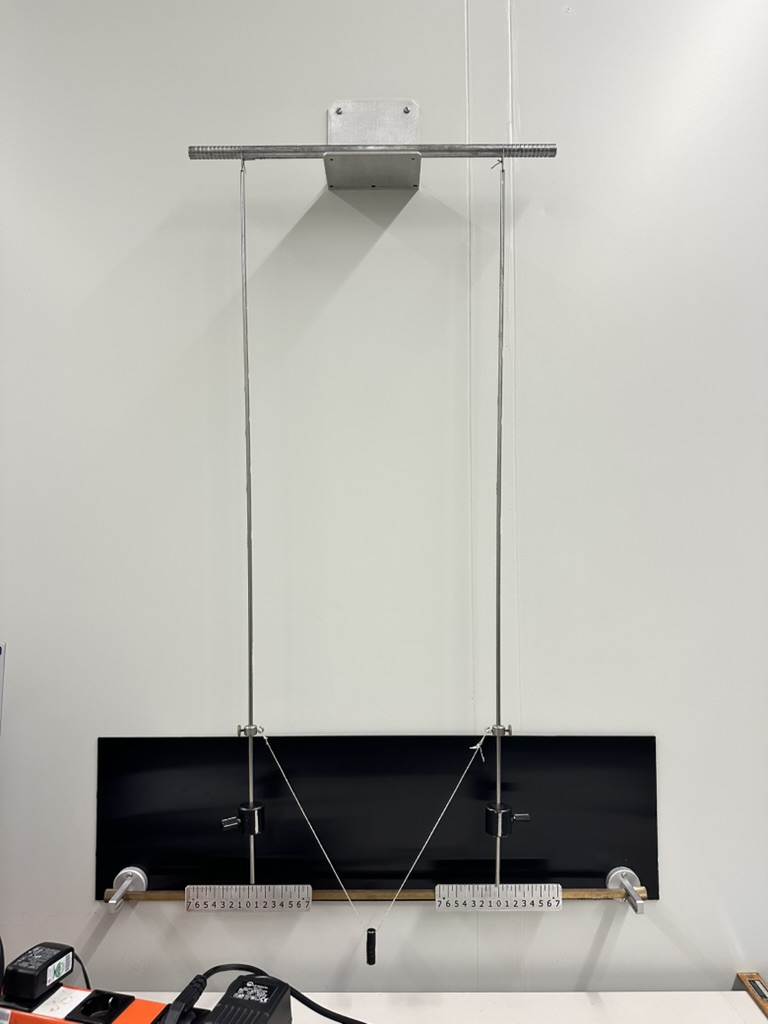
\includegraphics[width=0.4\textwidth]{Aufbau}}
	\caption{Aufbau der Pendel, die hier bei \(\lh = \qty{70}{\centi\meter}\) gekoppelt sind.}
	\label{fig:aufbau}
\end{figure}



\section[Formeln]{Formeln}

\section{Messwerte}

\begin{table}[H]
	\begin{tabular*}{\textwidth}{@{\extracolsep{\fill}}@{\hspace{5pt}}lrr@{\hspace{5pt}}}
		\toprule
		Parameter & Pendel \num{1} & Pendel \num{2}\\
		\midrule
		Masse des Pendelkörpers \(m\)\,/\,\si{\kilogram} & \num{176,97e-3}   & \num{174,95e-3}\\
		Masse des Hakens \(m_{\text{H}}\)\,/\,\si{\kilogram} & \num{16,06e-3}   & \num{15,80e-3}\\
		Masse der Stange & \num{131,40e-3} & \num{131,27e-3}\\
		\(L\)\,/\, \si{\kilogram} & \num{0,804} & \num{0,800}\\
		\(\lh\) \,/\, \si{\meter} & \num{0,4} & \num{0,4}\\
		\(L_{\text{St}}\)\,/\, \si{\meter} & \num{0,87} & \num{0,87}\\
		\bottomrule
	\end{tabular*}
	\caption{Ungekoppelter gleichsinniger Fall \label{tbl:dimensions}}
\end{table}

\subsection{\texorpdfstring{\qty{40}{\centi\meter}}{40 cm}}

\begin{table}[H]
	\begin{tabular*}{\textwidth}{@{\extracolsep{\fill}}@{\hspace{5pt}}lrr@{\hspace{5pt}}}
		\toprule
		Pendel & \(t_0\)\,/\,\(\si{\second}\) & \(t_1\)\,/\,\(\si{\second}\)\\
		\midrule
		1 & \num{1,4}   & \num{35,5}\\
		2 & \num{1,3}   & \num{35,4}\\
		\bottomrule
	\end{tabular*}
	\caption{Ungekoppelter gleichsinniger Fall \label{tbl:ngekgl40}}
\end{table}

\begin{table}[H]
	\begin{tabular*}{\textwidth}{@{\extracolsep{\fill}}@{\hspace{5pt}}lrr@{\hspace{5pt}}}
		\toprule
		Pendel & \(t_0\)\,/\,\(\si{\second}\) & \(t_1\)\,/\,\(\si{\second}\)\\
		\midrule
		1 & \num{0,9}   & \num{34,8}\\
		2 & \num{0,8}   & \num{34,8}\\
		\bottomrule
	\end{tabular*}
	\caption{Gekoppelter gleichsinniger Fall \label{tbl:gekgl40}}
\end{table}

\begin{table}[H]
	\begin{tabular*}{\textwidth}{@{\extracolsep{\fill}}@{\hspace{5pt}}lrr@{\hspace{5pt}}}
		\toprule
		Pendel & \(t_0\)\,/\,\(\si{\second}\) & \(t_1\)\,/\,\(\si{\second}\)\\
		\midrule
		1 & \num{0,4}   & \num{33,3}\\
		2 & \num{1,2}   & \num{34,1}\\
		\bottomrule
	\end{tabular*}
	\caption{Gekoppelter gegensinniger Fall \label{tbl:gekgeg40}}
\end{table}

\begin{table}[H]
	\begin{tabular*}{\textwidth}{@{\extracolsep{\fill}}@{\hspace{5pt}}lrrrrr@{\hspace{5pt}}}
		\toprule
		Pendel & \(t_0\)\,/\,\(\si{\second}\) & \(t_1\)\,/\,\(\si{\second}\)& \(t_2\)\,/\,\(\si{\second}\)& \(t_3\)\,/\,\(\si{\second}\)& \(t_4\)\,/\,\(\si{\second}\)\\
		\midrule
		1 & \num{0,0}   & \num{52,4} & \num{105,8} & \num{160,0} & \num{211,6}\\
		2 & \num{25,4}   & \num{79,5} & \num{132,9} & \num{185,3} & \num{237,8}\\
		\bottomrule
	\end{tabular*}
	\caption{Schwebungsfall \label{tbl:schweb40}}
\end{table}

\subsection{\texorpdfstring{\qty{55}{\centi\meter}}{55 cm}}

\begin{table}[H]
	\begin{tabular*}{\textwidth}{@{\extracolsep{\fill}}@{\hspace{5pt}}lrr@{\hspace{5pt}}}
		\toprule
		Pendel & \(t_0\)\,/\,\(\si{\second}\) & \(t_1\)\,/\,\(\si{\second}\)\\
		\midrule
		1 & \num{0,8}   & \num{35,0}\\
		2 & \num{0,8}   & \num{34,8}\\
		\bottomrule
	\end{tabular*}
	\caption{Ungekoppelter gleichsinniger Fall \label{tbl:ngekgl55}}
\end{table}

\begin{table}[H]
	\begin{tabular*}{\textwidth}{@{\extracolsep{\fill}}@{\hspace{5pt}}lrr@{\hspace{5pt}}}
		\toprule
		Pendel & \(t_0\)\,/\,\(\si{\second}\) & \(t_1\)\,/\,\(\si{\second}\)\\
		\midrule
		1 & \num{0,5}   & \num{34,5}\\
		2 & \num{0,5}   & \num{34,5}\\
		\bottomrule
	\end{tabular*}
	\caption{Gekoppelter gleichsinniger Fall \label{tbl:gekgl55}}
\end{table}

\begin{table}[H]
	\begin{tabular*}{\textwidth}{@{\extracolsep{\fill}}@{\hspace{5pt}}lrr@{\hspace{5pt}}}
		\toprule
		Pendel & \(t_0\)\,/\,\(\si{\second}\) & \(t_1\)\,/\,\(\si{\second}\)\\
		\midrule
		1 & \num{1,4}   & \num{33,6}\\
		2 & \num{0,6}   & \num{32,9}\\
		\bottomrule
	\end{tabular*}
	\caption{Gekoppelter gegensinniger Fall \label{tbl:gekgeg55}}
\end{table}

\begin{table}[H]
	\begin{tabular*}{\textwidth}{@{\extracolsep{\fill}}@{\hspace{5pt}}lrrrrr@{\hspace{5pt}}}
		\toprule
		Pendel & \(t_0\)\,/\,\(\si{\second}\) & \(t_1\)\,/\,\(\si{\second}\)& \(t_2\)\,/\,\(\si{\second}\)& \(t_3\)\,/\,\(\si{\second}\)& \(t_4\)\,/\,\(\si{\second}\)\\
		\midrule
		1 & \num{14,8}   & \num{44,9} & \num{74,6} & \num{105,2} & \num{134,8}\\
		2 & \num{0,0}   & \num{29,5} & \num{60,2} & \num{89,8} & \num{119,6}\\
		\bottomrule
	\end{tabular*}
	\caption{Schwebungsfall \label{tbl:schweb55}}
\end{table}

\subsection{\texorpdfstring{\qty{70}{\centi\meter}}{70 cm}}

\begin{table}[H]
	\begin{tabular*}{\textwidth}{@{\extracolsep{\fill}}@{\hspace{5pt}}lrr@{\hspace{5pt}}}
		\toprule
		Pendel & \(t_0\)\,/\,\(\si{\second}\) & \(t_1\)\,/\,\(\si{\second}\)\\
		\midrule
		1 & \num{1,5}   & \num{35,8}\\
		2 & \num{1,5}   & \num{35,7}\\
		\bottomrule
	\end{tabular*}
	\caption{Ungekoppelter gleichsinniger Fall \label{tbl:ngekgl70}}
\end{table}

\begin{table}[H]
	\begin{tabular*}{\textwidth}{@{\extracolsep{\fill}}@{\hspace{5pt}}lrr@{\hspace{5pt}}}
		\toprule
		Pendel & \(t_0\)\,/\,\(\si{\second}\) & \(t_1\)\,/\,\(\si{\second}\)\\
		\midrule
		1 & \num{0,5}   & \num{34,7}\\
		2 & \num{0,5}   & \num{34,7}\\
		\bottomrule
	\end{tabular*}
	\caption{Gekoppelter gleichsinniger Fall \label{tbl:gekgl70}}
\end{table}

\begin{table}[H]
	\begin{tabular*}{\textwidth}{@{\extracolsep{\fill}}@{\hspace{5pt}}lrr@{\hspace{5pt}}}
		\toprule
		Pendel & \(t_0\)\,/\,\(\si{\second}\) & \(t_1\)\,/\,\(\si{\second}\)\\
		\midrule
		1 & \num{1,5}   & \num{33,0}\\
		2 & \num{0,7}   & \num{32,2}\\
		\bottomrule
	\end{tabular*}
	\caption{Gekoppelter gegensinniger Fall \label{tbl:gekgeg70}}
\end{table}

\begin{table}[H]
	\begin{tabular*}{\textwidth}{@{\extracolsep{\fill}}@{\hspace{5pt}}lrrrrr@{\hspace{5pt}}}
		\toprule
		Pendel & \(t_0\)\,/\,\(\si{\second}\) & \(t_1\)\,/\,\(\si{\second}\)& \(t_2\)\,/\,\(\si{\second}\)& \(t_3\)\,/\,\(\si{\second}\)& \(t_4\)\,/\,\(\si{\second}\)\\
		\midrule
		1 & \num{0,0}   & \num{18,1} & \num{38,7} & \num{58,3} & \num{77,8}\\
		2 & \num{9,0}   & \num{29,5} & \num{49,0} & \num{68,6} & \num{88,3}\\
		\bottomrule
	\end{tabular*}
	\caption{Schwebungsfall \label{tbl:schweb70}}
\end{table}

\begin{table}[H]
	\begin{tabular*}{\textwidth}{@{\extracolsep{\fill}}@{\hspace{5pt}}lrrrrr@{\hspace{5pt}}}
		\toprule
		Pendel & \(t_0\)\,/\,\(\si{\second}\) & \(t_1\)\,/\,\(\si{\second}\)& \(t_2\)\,/\,\(\si{\second}\)& \(t_3\)\,/\,\(\si{\second}\)& \(t_4\)\,/\,\(\si{\second}\)\\
		\midrule
		1 & \num{6,2}   & \num{26,7} & \num{47,1} & \num{66,9} & \num{85,6}\\
		2 & \num{16,4}   & \num{36,9} & \num{57,3} & \num{77,1} & \num{97,4}\\
		\bottomrule
	\end{tabular*}
	\caption{Schwebungsfall für unterschiedlich ausgelenkte Massen \label{tbl:schwebX70}}
\end{table}

\section{Auswertung}

\(T_0\) berechnet sich aus den Daten, die in \autoref{tbl:ngekgl40} eingetragen sind durch
\begin{equation}
	T_0 = \frac{t_1 - t_0}{20} \,,
\end{equation}
da zwischen \(t_0\) und \(t_1\) \num{20} Perioden durchlaufen wurden.
Damit ergibt sich für Pendel \num{1}
\begin{equation}
	T_{0,1} = \frac{\qty{35,5}{\second} - \qty{1,4}{\second}}{20} = \qty{1,7}{\second}
\end{equation}
und für Pendel \num{2} analog  ebenfalls \(T_{0,2} =\qty{1,7}{\second}\).

Für den Kopplungsgrad mit \(\lh = \qty{40}{\centi\meter}\) ergeben sich folgende Periodendauern.

\begin{table}[H]
	\begin{tabular*}{\textwidth}{@{\extracolsep{\fill}}@{\hspace{5pt}}lrrr@{\hspace{5pt}}}
		\toprule
		Periodendauer & Links & Rechts & Mittel\\
		\midrule
		\(T_{\text{gl}}\) & \qty{1,7}{\second} & \qty{1,7}{\second} & \qty{1,7}{\second}\\
		\(T_{\text{geg}}\) & \qty{1,6}{\second} & \qty{1,6}{\second} & \qty{1,6}{\second}\\
		\(T_{\text{II}}\) & \qty{1,6}{\second} & \qty{1,6}{\second} & \qty{1,6}{\second}\\
		\(T_{\text{S}}\) & \qty{52,9}{\second} & \qty{53,1}{\second} & \qty{53,0}{\second} \\
		\bottomrule
	\end{tabular*}
	\caption{Periodendauern für \(\lh\) \label{tbl:res40}}
\end{table}

Für den Kopplungsgrad mit \(\lh = \qty{55}{\centi\meter}\) ergeben sich folgende Periodendauern.

\begin{table}[H]
	\begin{tabular*}{\textwidth}{@{\extracolsep{\fill}}@{\hspace{5pt}}lrrr@{\hspace{5pt}}}
		\toprule
		Periodendauer & Links & Rechts & Mittel\\
		\midrule
		\(T_{\text{gl}}\) & \qty{1,7}{\second} & \qty{1,7}{\second} & \qty{1,7}{\second}\\
		\(T_{\text{geg}}\) & \qty{1,6}{\second} & \qty{1,6}{\second} & \qty{1,6}{\second}\\
		\(T_{\text{II}}\) & \qty{1,6}{\second} & \qty{1,6}{\second} & \qty{1,6}{\second}\\
		\(T_{\text{S}}\) & \qty{30,0}{\second} & \qty{29,9}{\second} & \qty{30,0}{\second} \\
		\bottomrule
	\end{tabular*}
	\caption{Periodendauern für \(\lh\) \label{tbl:res55}}
\end{table}

Für den Kopplungsgrad mit \(\lh = \qty{70}{\centi\meter}\) ergeben sich folgende Periodendauern.

\begin{table}[H]
	\begin{tabular*}{\textwidth}{@{\extracolsep{\fill}}@{\hspace{5pt}}lrrr@{\hspace{5pt}}}
		\toprule
		Periodendauer & Links & Rechts & Mittel\\
		\midrule
		\(T_{\text{gl}}\) & \qty{1,7}{\second} & \qty{1,7}{\second} & \qty{1,7}{\second}\\
		\(T_{\text{geg}}\) & \qty{1,6}{\second} & \qty{1,6}{\second} & \qty{1,6}{\second}\\
		\(T_{\text{II}}\) & \qty{1,6}{\second} & \qty{1,6}{\second} & \qty{1,6}{\second}\\
		\(T_{\text{S}}\) & \qty{19,5}{\second} & \qty{19,8}{\second} & \qty{19,6}{\second} \\
		\bottomrule
	\end{tabular*}
	\caption{Periodendauern für \(\lh\) \label{tbl:res70}}
\end{table}

\begin{figure}[H]
	\centering{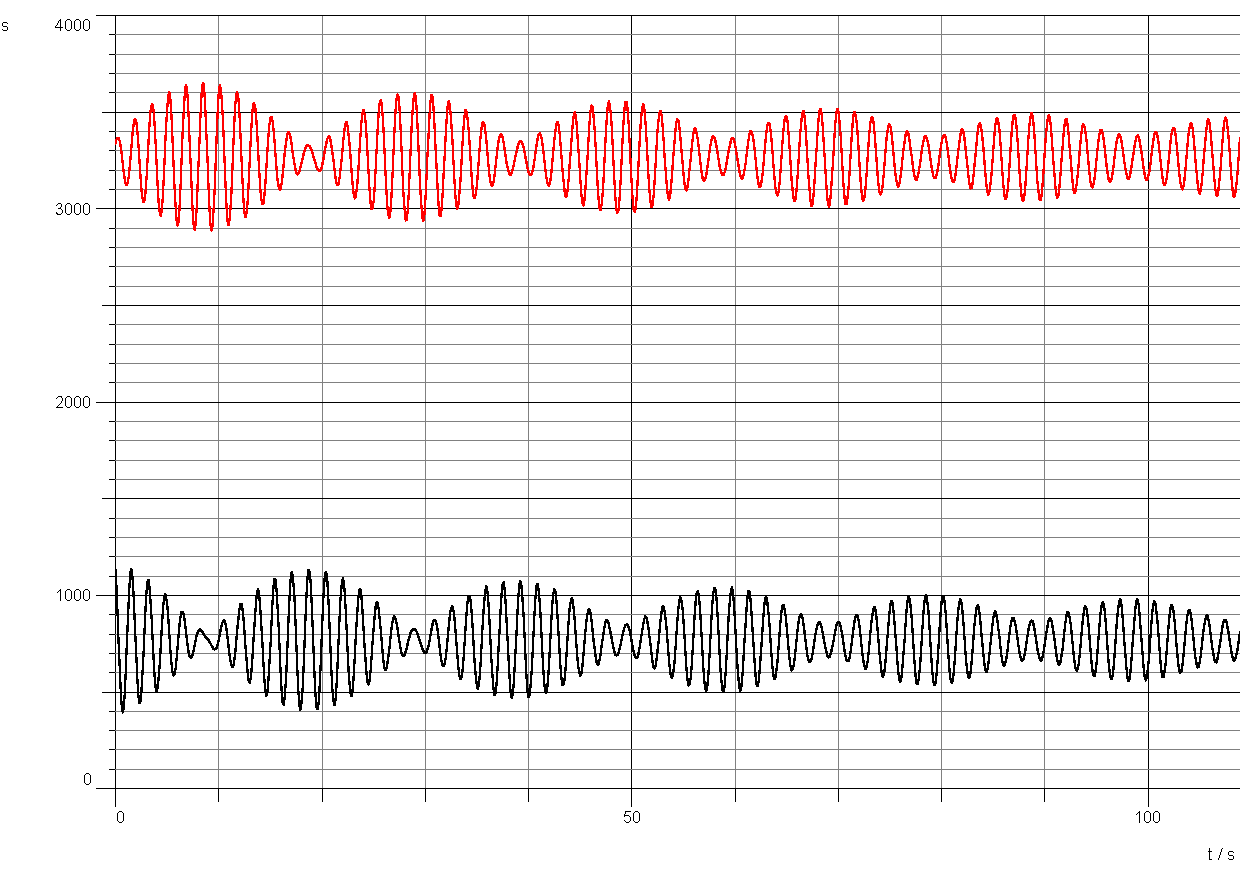
\includegraphics[width=0.9\textwidth]{SCHWEBUNG_70cm.pdf}}
	\caption{Exemplarisches \(x(t)\)-Diagramm des Schwebungsfalles bei \(\lh = \qty{70}{\centi\meter}\)}
	\label{fig:schweb}
\end{figure}

\begin{figure}[H]
	\centering{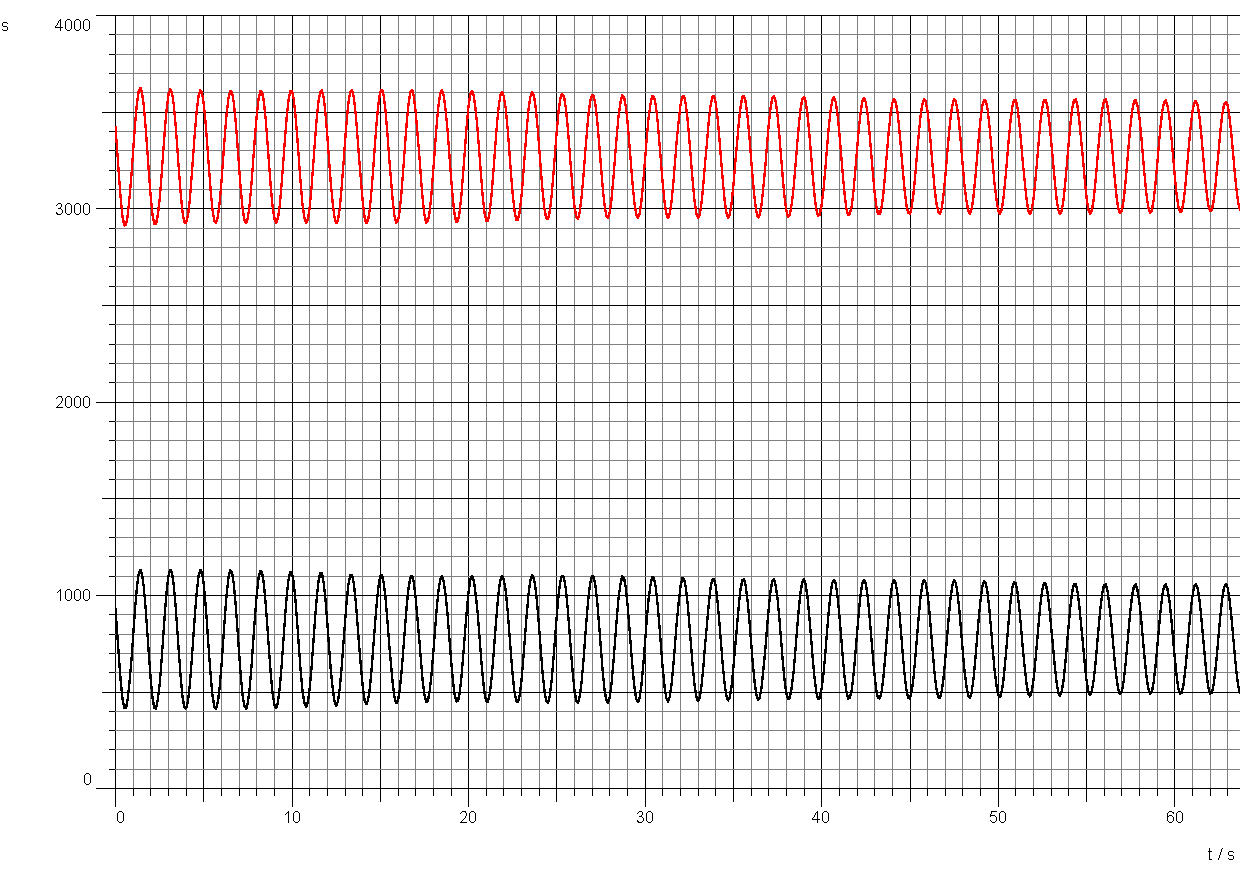
\includegraphics[width=0.9\textwidth]{gleichsinnige_FUNDAMENTALSCHWINGUNG_70cm.pdf}}
	\caption{Exemplarisches \(x(t)\)-Diagramm der gleichsinnigen Fundamentalschwingung bei \(\lh = \qty{70}{\centi\meter}\)}
	\label{fig:gl70}
\end{figure}

\begin{figure}[H]
	\centering{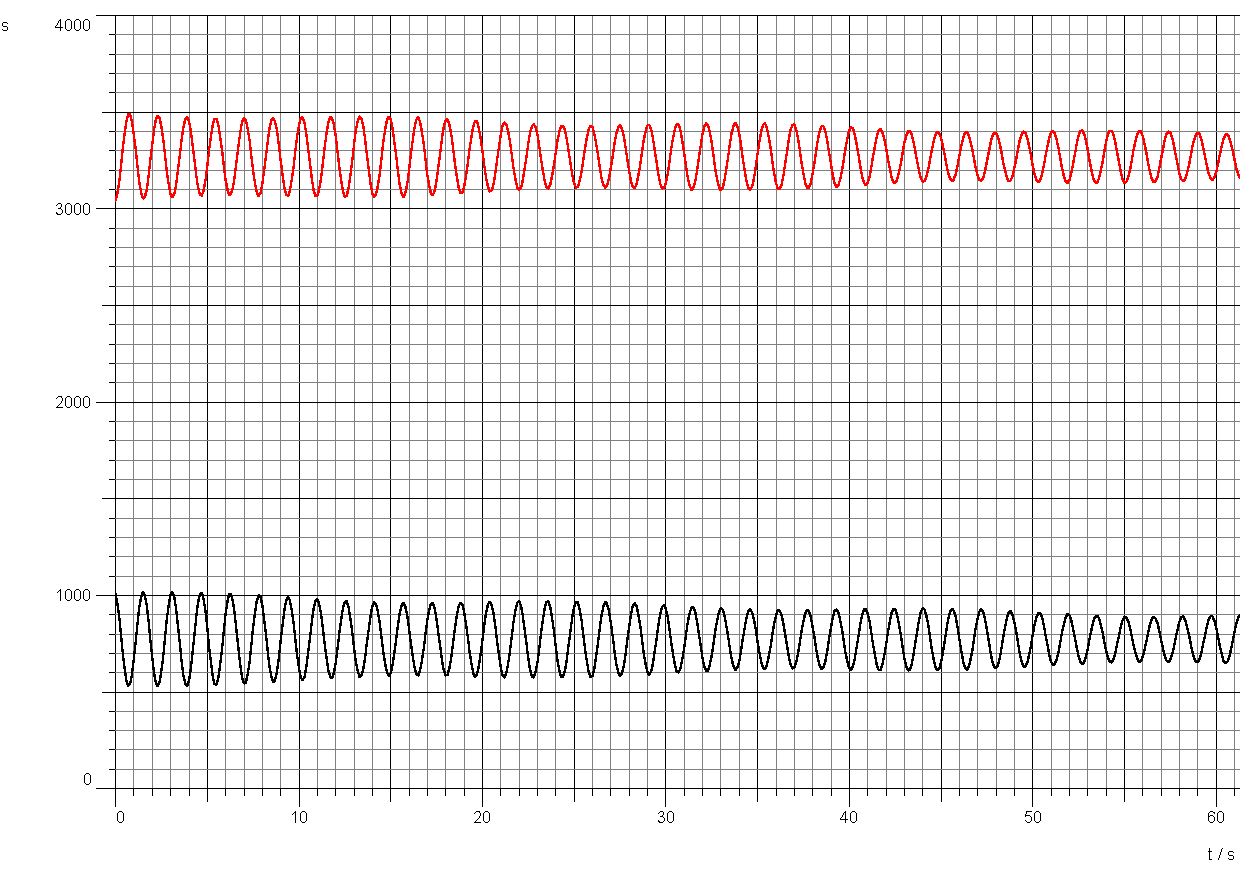
\includegraphics[width=0.9\textwidth]{gegensinnige_FUNDAMENTALSCHWINGUNG_70cm.pdf}}
	\caption{Exemplarisches \(x(t)\)-Diagramm der gegensinnigen Fundamentalschwingung bei \(\lh = \qty{70}{\centi\meter}\)}
	\label{fig:geg70}
\end{figure}


%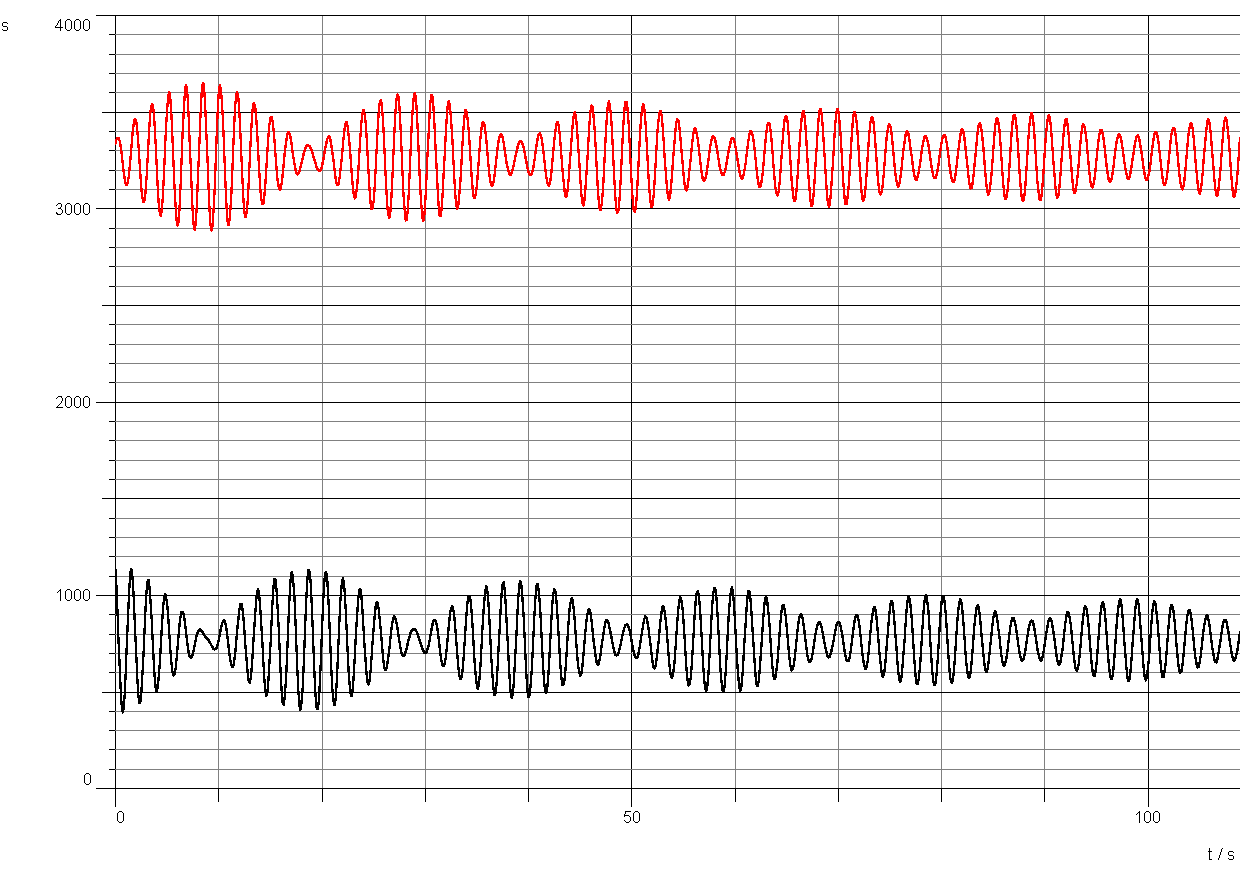
\includepdf[pages=-]{SCHWEBUNG_70cm.pdf}
%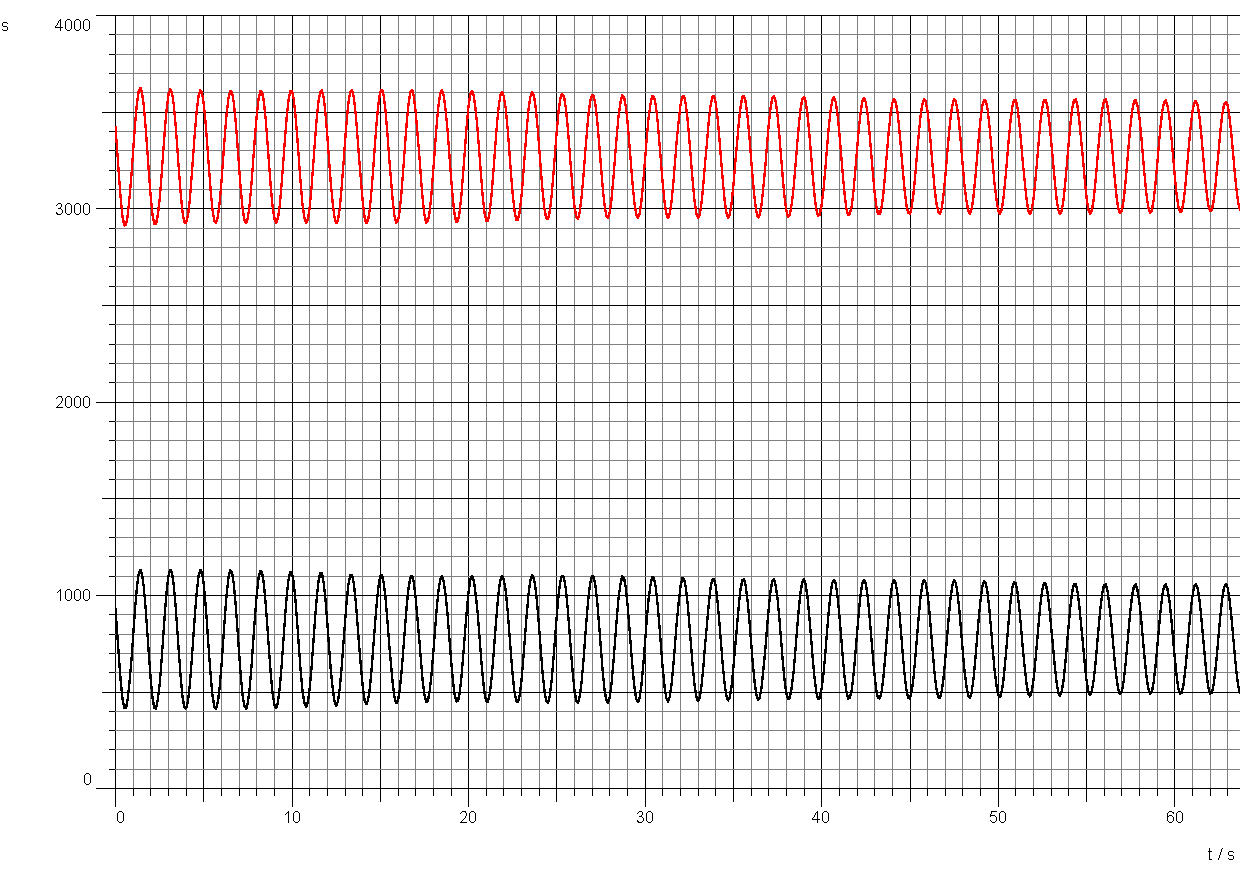
\includepdf[pages=-]{gleichsinnige_FUNDAMENTALSCHWINGUNG_70cm.pdf}
%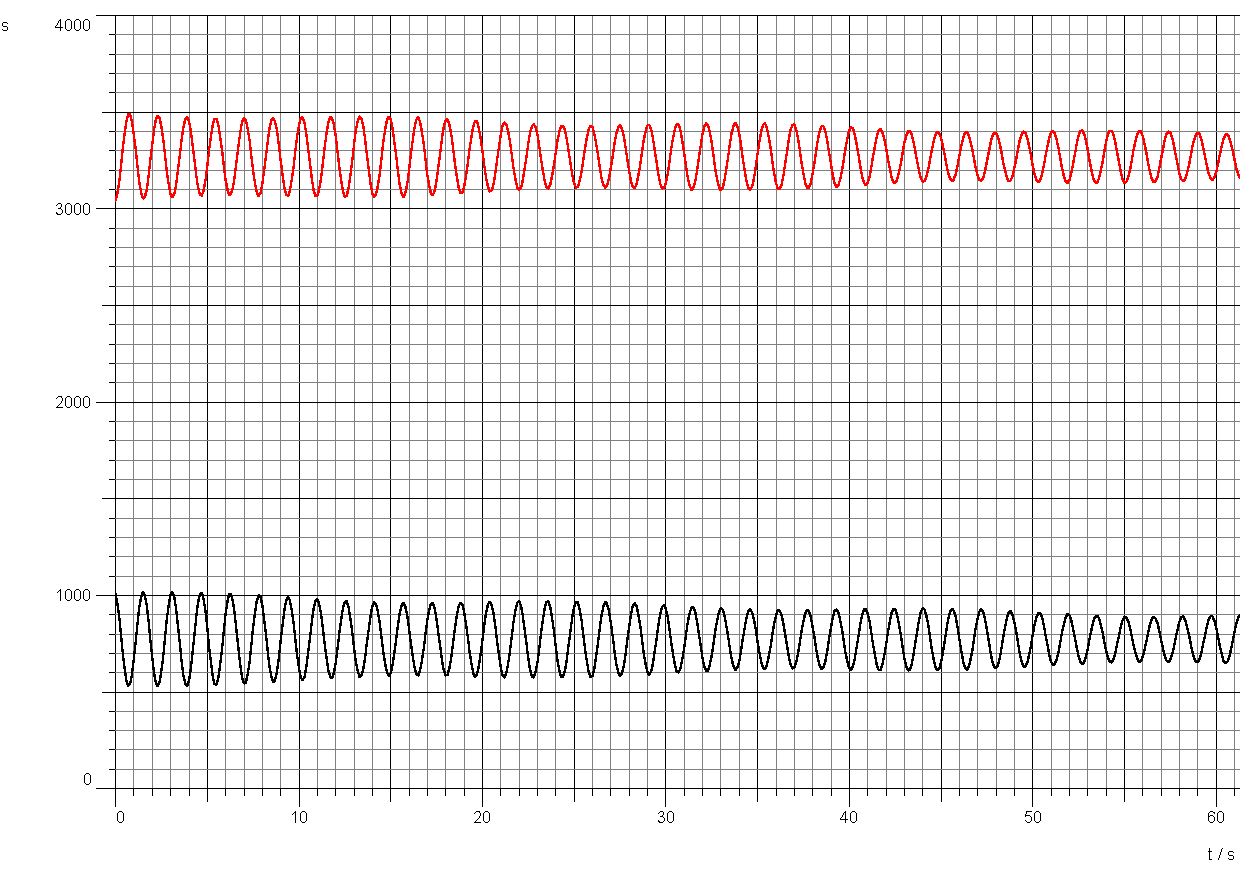
\includepdf[pages=-]{gegensinnige_FUNDAMENTALSCHWINGUNG_70cm.pdf}

Nach %\autoref{eq:Drehmoment}
wird das Gesamtträgheitsmoment mit den Daten aus \autoref{tbl:dimensions} berechnet. Für das erste Pendel ergibt sich das Trägheitsmoment
\begin{equation}
	\begin{split}
		J_1 = \frac{1}{3} \cdot \qty{131,40e-3}{\kilogram} \cdot (\qty{0,87}{\meter})^2 &+ \qty{16,06e-3}{\kilogram} \cdot (\qty{0,4}{\meter})^2
		\\&+ \qty{176,97e-3}{\kilogram} \cdot (\qty{0,804}{\meter})^2 = \qty{0,150}{\kilogram\meter\squared}
	\end{split}
\end{equation}
und für das zweite Pendel \(J_2 = \qty{0,148}{\kilogram\meter\squared}\).

Die Eigenfrequenz \(\omega_0\) wird mittels %\autoref{eq:eig}
berechnet. Dafür muss zuerst die Lage des Schwerpunktes \(\ls\) mit %\autoref{eq:schwerp}
berechnet werden und ergibt
\begin{equation}
	\ls = \frac{Lm + \lh m_{\text{H}} + \tfrac{1}{2} L_{\text{St}} m_{\text{St}}}{m + m_{\text{H}} + m_{\text{St}}}
\end{equation}
\begin{equation}
	\begin{split}
		\ell_{\text{S},1} &= \frac{\qty{0,804}{\meter} \cdot \qty{176,97e-3}{\kilogram} + \qty{0,4}{\meter} \cdot \qty{16,06e-3}{\kilogram} + \tfrac{1}{2}\qty{0,87}{\meter} \cdot \qty{131,40e-3}{\kilogram}}{\mleft(\num{176,97e-3} + \num{16,06e-3} + \num{131,40e-3}\mright)\si{\kilogram}}\\
		&= \qty{0,635}{\meter}
	\end{split}
\end{equation}
Für \(\ell_{\text{S},2}\) ergibt sich \(\ell_{\text{S},1} = \qty{0,632}{m}\).

\section{Fehlerrechnung}

\section{Zusammenfassung}


\begin{thebibliography}{999}
	\bibitem{Quelle} Versuchsanleitung zu (Abgerufen am 1.04.2050)
\end{thebibliography}


\section{Anhang}

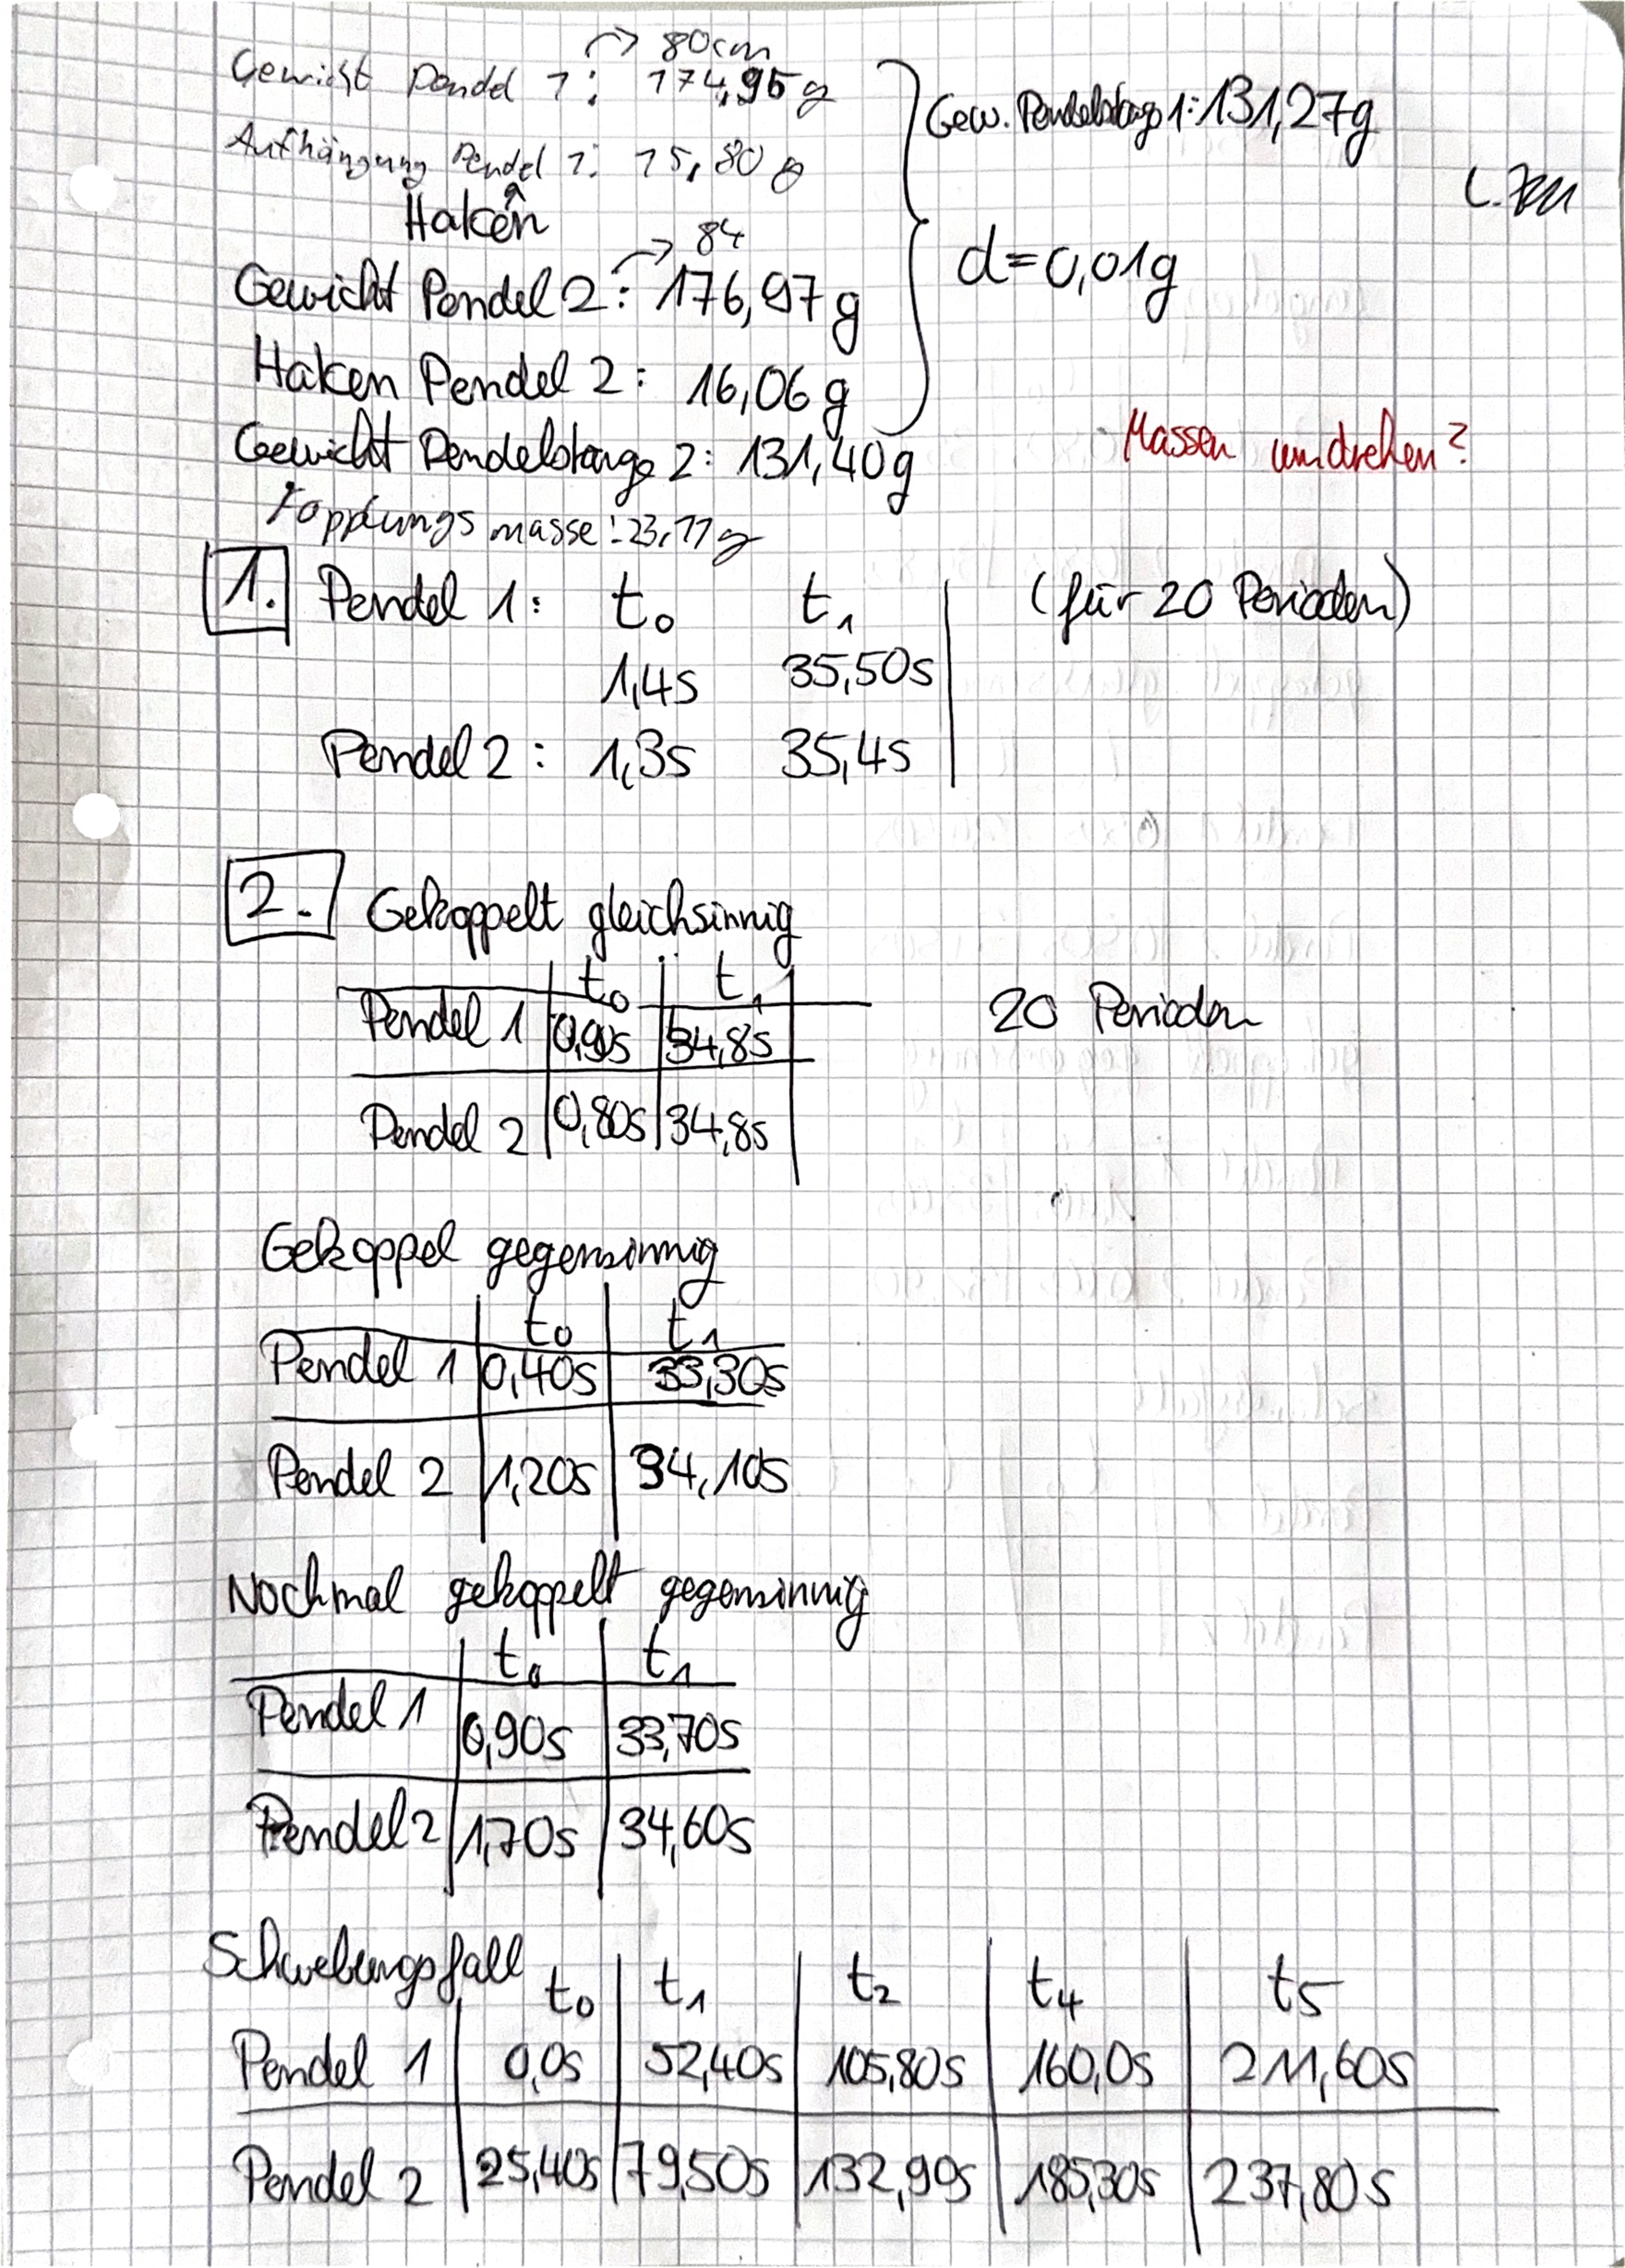
\includepdf[pages=-]{Messprotokoll.pdf}

\end{document}